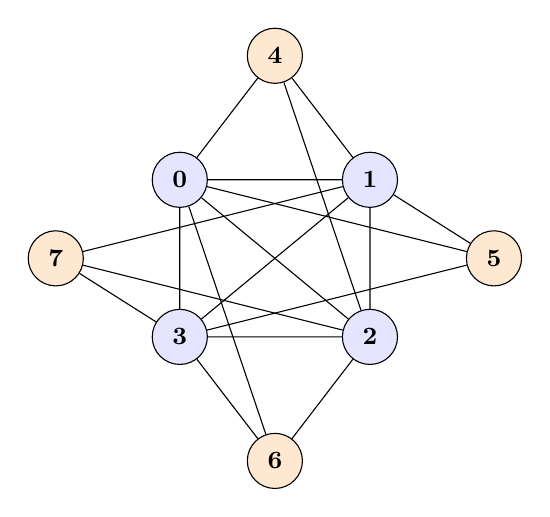
\begin{tikzpicture}[scale=1.05,
  core/.style={circle,draw=black,fill=blue!10,minimum size=7mm,inner sep=0pt,font=\small\bfseries},
  apex/.style={circle,draw=black,fill=orange!18,minimum size=7mm,inner sep=0pt,font=\small\bfseries},
  every edge/.style={draw=black!72,line width=.55pt}]
  \node[core] (v0) at (-1.15, 0.95) {0};
  \node[core] (v1) at ( 1.15, 0.95) {1};
  \node[core] (v2) at ( 1.15,-0.95) {2};
  \node[core] (v3) at (-1.15,-0.95) {3};
  \node[apex] (v4) at ( 0.00, 2.45) {4};
  \node[apex] (v5) at ( 2.65, 0.00) {5};
  \node[apex] (v6) at ( 0.00,-2.45) {6};
  \node[apex] (v7) at (-2.65, 0.00) {7};
  % Core K4: 01,02,03,12,13,23.
  \foreach \u/\v in {0/1,0/2,0/3,1/2,1/3,2/3}
    \draw (v\u) -- (v\v);
  % Apex 4 misses core 3; apex 5 misses 2; apex 6 misses 1; apex 7 misses 0.
  \foreach \u/\v in {4/0,4/1,4/2,5/0,5/1,5/3,6/0,6/2,6/3,7/1,7/2,7/3}
    \draw (v\u) -- (v\v);
\end{tikzpicture}
